\documentclass[11pt]{article}\usepackage[]{graphicx}\usepackage[]{color}
% maxwidth is the original width if it is less than linewidth
% otherwise use linewidth (to make sure the graphics do not exceed the margin)
\makeatletter
\def\maxwidth{ %
  \ifdim\Gin@nat@width>\linewidth
    \linewidth
  \else
    \Gin@nat@width
  \fi
}
\makeatother

\definecolor{fgcolor}{rgb}{0.345, 0.345, 0.345}
\newcommand{\hlnum}[1]{\textcolor[rgb]{0.686,0.059,0.569}{#1}}%
\newcommand{\hlstr}[1]{\textcolor[rgb]{0.192,0.494,0.8}{#1}}%
\newcommand{\hlcom}[1]{\textcolor[rgb]{0.678,0.584,0.686}{\textit{#1}}}%
\newcommand{\hlopt}[1]{\textcolor[rgb]{0,0,0}{#1}}%
\newcommand{\hlstd}[1]{\textcolor[rgb]{0.345,0.345,0.345}{#1}}%
\newcommand{\hlkwa}[1]{\textcolor[rgb]{0.161,0.373,0.58}{\textbf{#1}}}%
\newcommand{\hlkwb}[1]{\textcolor[rgb]{0.69,0.353,0.396}{#1}}%
\newcommand{\hlkwc}[1]{\textcolor[rgb]{0.333,0.667,0.333}{#1}}%
\newcommand{\hlkwd}[1]{\textcolor[rgb]{0.737,0.353,0.396}{\textbf{#1}}}%
\let\hlipl\hlkwb

\usepackage{framed}
\makeatletter
\newenvironment{kframe}{%
 \def\at@end@of@kframe{}%
 \ifinner\ifhmode%
  \def\at@end@of@kframe{\end{minipage}}%
  \begin{minipage}{\columnwidth}%
 \fi\fi%
 \def\FrameCommand##1{\hskip\@totalleftmargin \hskip-\fboxsep
 \colorbox{shadecolor}{##1}\hskip-\fboxsep
     % There is no \\@totalrightmargin, so:
     \hskip-\linewidth \hskip-\@totalleftmargin \hskip\columnwidth}%
 \MakeFramed {\advance\hsize-\width
   \@totalleftmargin\z@ \linewidth\hsize
   \@setminipage}}%
 {\par\unskip\endMakeFramed%
 \at@end@of@kframe}
\makeatother

\definecolor{shadecolor}{rgb}{.97, .97, .97}
\definecolor{messagecolor}{rgb}{0, 0, 0}
\definecolor{warningcolor}{rgb}{1, 0, 1}
\definecolor{errorcolor}{rgb}{1, 0, 0}
\newenvironment{knitrout}{}{} % an empty environment to be redefined in TeX

\usepackage{alltt}

\usepackage{rotating}
\usepackage{graphics}
\usepackage{latexsym}
\usepackage{color}
\usepackage{listings}
\usepackage{wrapfig}
\usepackage{float}
\usepackage[belowskip=-15pt,aboveskip=0pt]{caption}

\setlength\topmargin{-.56in}
\setlength\evensidemargin{0in}
\setlength\oddsidemargin{0in}
\setlength\textwidth{6.49in}
\setlength\textheight{8.6in}
\setlength{\intextsep}{10pt plus 1pt minus 4pt}

\definecolor{codegreen}{rgb}{0,0.6,0}
\definecolor{codegray}{rgb}{0.5,0.5,0.5}
\definecolor{codepurple}{rgb}{0.58,0,0.82}
\definecolor{backcolour}{rgb}{0.95,0.95,0.92}
\lstdefinestyle{mystyle}{
	backgroundcolor=\color{backcolour},   
	commentstyle=\color{codegreen},
	keywordstyle=\color{magenta},
	numberstyle=\tiny\color{codegray},
	stringstyle=\color{codepurple},
	basicstyle=\footnotesize,
	breakatwhitespace=false,         
	breaklines=true,                 
	captionpos=b,                    
	keepspaces=true,                 
	numbers=left,                    
	numbersep=5pt,                  
	showspaces=false,                
	showstringspaces=false,
	showtabs=false,                  
	tabsize=2
}
\lstset{style=mystyle}

\pagestyle{headings}

\title{Predictive Model for Average Avocado Prices\vspace{-5ex}} 
\date{December 16, 2020\vspace{-5ex}}
\IfFileExists{upquote.sty}{\usepackage{upquote}}{}
\begin{document} 
\maketitle
\hfill \break
















\noindent\textbf{\underline{Executive Summary}}:      
\hfill \break

\noindent\textbf{\underline{Introduction}}: Avocado is a fruit that is originated from southern America. This fruit is extremaly health and have a lot of benefits and nutritions. Individuals can use avocados with any other ingridients to complete a meal such as toast and salad. In addition, avocados can also be used to make healthy oil or desserts like avocado ice cream or smoothie. Knowing the fact that avocados are health for a human body, avocados have been the rise of American's new favorites fruits since the last decade. The amount of avocados have been sold in America are higher and higher everyday. With this being said, knowing the variables that cause the price of avocados to go up and down would benefits all consumers and restaurants owner. For example, a restaurants that have avocado toast or guacamole on their menu would have a better understanding of where to get cheaper avocados to maximize their profit. Knowing the cost of avocado can also help restaurants owner create budget for their restaurant and cost of a dish on their menu. In addition, individuals who like avocado would also know where and when to get type of avocado they desire. There are many questions asked in favor of these issues including 1) What factor impact the average price of avocados? 2) Are characteristics of an avocado important in pricing decision? 3) How good is the model? 4) How can we improve the model? and 5) How can we implement the model for the consumer to gain easy access? This analysis will attempt to answer all these questions by starting with a variable data analysis, developing the model using a multiple linear regression, assessing the quality of the model, and providing significant results of the model. The purpose of this model is to predict the average avocado prices using various variables provided in the dataset.         
\hfill \break

\noindent\textbf{\underline{Methods}}: A dataset was retrieved from Kaggle, a website that have input and output from scientists and college students. This dataset has a large sample size of 30,021 observations from 2015 to 2020. The data was originally collected from the Hass Avocado Broad (HAB) website. There are no missing values for all the variables in the dataset. This dataset has historical data of avocado prices and characteristics. The dataset contains two time series columns including date of observation and year of observation, one characteristic variable including type of the avocado, and one geographical variable. In addition, there are eight quantitative predictors including total number of avocados sold, total number of avocados with Price Look-Up (PLU) code 4046 sold, total number of avocados with PLU code 4226 sold, total number of avocados with PLU code 4770 sold, total number of bags sold, total number of small bags sold, total number of large bags sold, and total number of extra large bags sold. There are 54 distinct geographical regions of where the avocados are from with different average prices for different time of the year. The goal of this analysis is to find the relationship between predictors and average avocado prices. To build a model with average avocado price, a multiple linear regression with signficant predictors will be used. Before building a model, we will explore how each variable impact the average of avocado prices. Then, using the "best" model, we will predict the avocado price to validate our model. The data will be splitted into a .75/.25 proportion train/test set. All analysis will be done in R Studio with version 3.6.2.  
\hfill \break

\noindent\textbf{\underline{Exploratory Data Analysis}}: Before building a model, it is important to explore the distribution of average avocado prices and the relationship of it with each of the predictor. The target variable average price have an approximately normal distribution, see Figure~\ref{explore1}.1. With a normal distribution assumption, a multiple linear regression can be applied. The price of avocados range from \$0.44 to \$3.25 with an average of \$1.35 for each avocado. In terms of predictors, a descriptive statistics was constructed for all continuous variable in the dataset, see Table~A\ref{desc_stat_ind} in the Appendix. All continuous variable are right skewed with an extremely large maximum value compare to the means and the third interquatile ranges. This signifies a log-transformation is needed for all continous predictors to minimize skewness effect. In addition, the values of the continuous variables will be smaller and easier to analyze.      

\begin{figure}[h!] 
\begin{center}

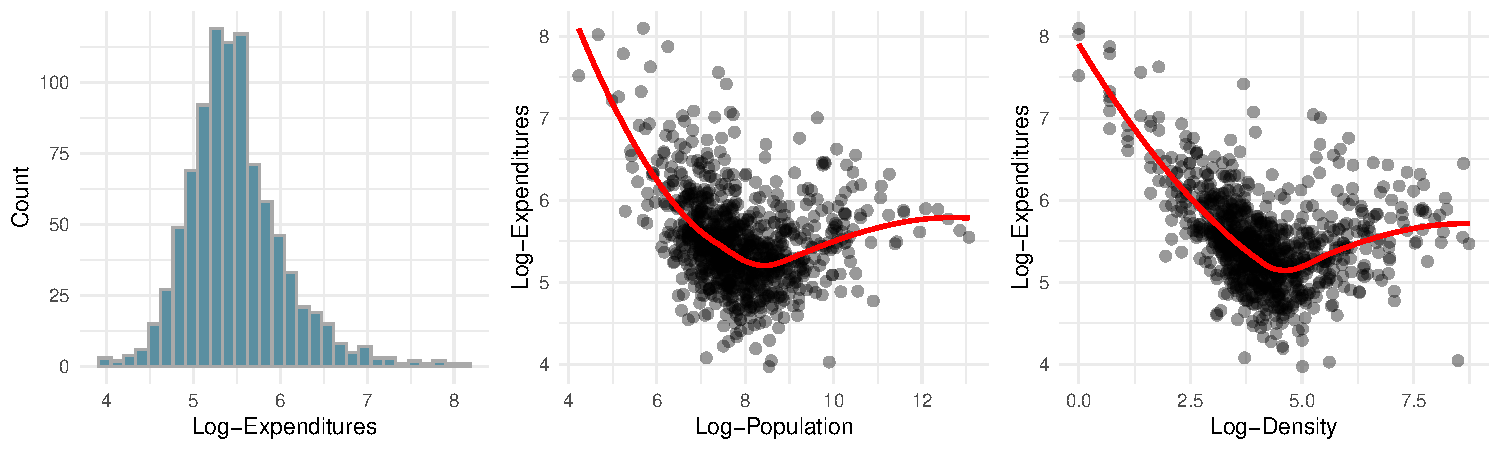
\includegraphics[width=\maxwidth]{figure/unnamed-chunk-1-1} 

\caption{}
\label{explore1}
\end{center} 
\end{figure}

\noindent Total number of avocados sold is the number that have been sold in each location and each time of the year. Economically, the price of avocado will be lower if there are more supply. On the other hand, the price will be higher if there is a shortage in avocado. On a consumer side, a cheaper avocado would be more like to be bought than a more expensive one. This leads to a higher sells in avocados if the price is cheaper. Figure~\ref{explore1}.2 shows a negative relationship between average avocado price and the log-transformation of total number of avocados sold. The rest of the article will use log of total number of avocados sold, unless otherwise specify. In Figure~\ref{explore1}.2, the total number of avocados sold were sorted from smallest to highest and divided into 10 equal buckets. The first bucket contains the smaller number of avocados solds. The last bucket contains the highest number of avocados sold. A negative relationship indicates the average price will be cheaper if there are more avocado sold. However, the price will be more expensive if there are less avocado sold. This have proven the points of less supply lead to higher price. Likewise, higher price of avocados leads to less consumpsion. Therefore, the amount of avocado sold will be less. This variable would contribute significant impact in the model to predict the averge of avocado prices.  
\hfill \break

\noindent The type of the avocado is also a signicant factor that would change the price of an avocado. In this dataset, there are two types of avocados including conventional and organic. Conventional avocados are traditoinal growing method that majority of the countries do. The price of conventional avocado would be more likely to be cheaper since the cost of growing conventional avocados are cheaper. On the other hand, organic avocados are growed without using any chemical, fertilizers, pesticides, or other artificial agents. Without a booster, organic avovados take longer to grow and easier to be eaten by insects. Therefore, the price of organic avocado would be considered more expensive. Figure~\ref{explore1}.3 depicts the relationship of average avocado price with avocado types. As seen in the plot shown using a black line, organic avocados have a higher average price than conventional avocado. This indicates that an organic avocado would cause the price to be higher compared to a conventional avocado. Furthermore, this variable, type of avocado, have a balance proportion (shown using two bars). With a balance proportion, the predictive model would be more unbiased. Therefore, type of avocados would contribute a significant impact in predicting the price of avocados.      
\hfill \break

\noindent Month of observation is the time where the avocado is observed. Time of the year is important for fruits and vegitables because majority of the fruit only grow in a certain months or their season. Therefore, we would expect to have more avocados during avocado season and less avocados otherwise. As mentioned before, the price of avocado would be more like to increase if there are less avocados in supply. This means that, the average price would increase during non-avocado seasons and decrease during avocado seasons. Figure~\ref{explore2}.1 shows a plot of average avocado price by month of observation with its frequency. As one can see, avocado seasons can be assume to be between January and May with the highest number of observations. On the other hand, non-avocado seasons are likely to be in between the month of June to December with lower number of avocados observed. In addition, a black line depicts lower average prices from January to May and higher prices from June to December. This indicates that during avocados season, the price of avocados are lower because there are more avocados in supply. On the other hand, the low supply of avocados from June to December causes the average price to go up. Therefore, this variable month of the year could contribute significant relationship with average price in the linear regression model.


\begin{figure}[h!] 
\begin{center}

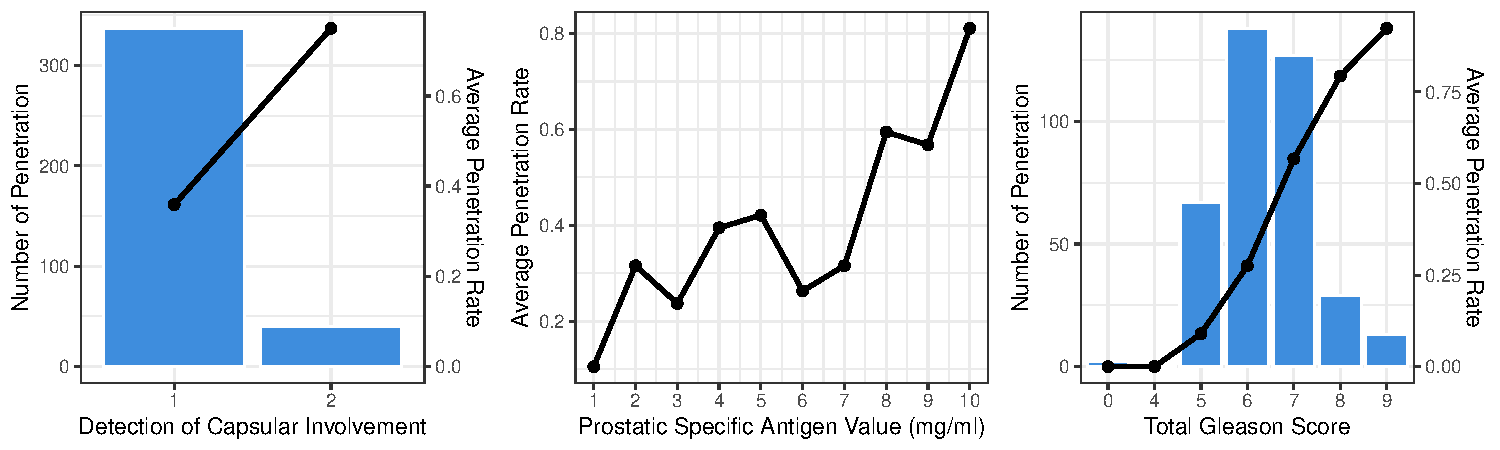
\includegraphics[width=\maxwidth]{figure/unnamed-chunk-2-1} 

\caption{}
\label{explore2}
\end{center} 
\end{figure}

Last but not least, location of the avocados sold could also be significant to the model. The geography of the avocado is the region or city the avocado is sold. Different cities and states have different living expenses resulting in different prices of the avocados. For example, the living expenses in California is higher than Texas. Thus, the price of avocados in California cities would be higher than the prices of avocados in Texas. Figure~\ref{explore2}.2 depicts a relationship between average avocado prices and geographical location. This variables is sorted from smallest to highest average price and assign four geographical group. The first geographical group sells cheapest avocados. The regions in the first group include Cincinnati, Columbus, Dallas, Houston, Nashville, New Orleans, Phoenix, Roanoke, and South Central. Furthermore, the last geographical group sells the most expensive avocados. Those regions include Hartford, New York, and San Francisco. Knowing the location of the market, the model can provide more variation of the average price.         
\hfill \break

Other variables like total number of avocados with Price Look-Up (PLU) code 4046 sold, total number of avocados with PLU code 4226 sold, total number of avocados with PLU code 4770 sold, total number of bags sold, total number of small bags sold, total number of large bags sold, and total number of extra large bags sold also have a strong negative relationship with the average prices. However, the correlation of all the continuous independent variable are very high, majority above .80, see Figure~\ref{explore2}.3. If all high correlated variables are used within the same model, multicolinarity issues will arise. This leads the coefficients of each predictors to be unstable. Therefore, only total number of avocados sold will be use in the model. Total volume would describe total number of all different categories added up. In other words, the variables total number of avocados with Price Look-Up (PLU) code 4046 sold, total number of avocados with PLU code 4226 sold, total number of avocados with PLU code 4770 sold, total number of bags sold, total number of small bags sold, total number of large bags sold, and total number of extra large bags sold are a component of total volume. Using just one variable total volume alone would be good enough to cover the details of each components. Other variables did not mentions in the exploratory analysis have little to no relationship with avaerage avocado prices.  
\hfill \break




\noindent\textbf{\underline{Model Fitting/Inferences}}: Now that we have found all the significant variables to predict the average price of avocados, predictive models can be achieved. As mentioned before, a train set of .75 of the proportion of the data was used to train train the models. The data splitting process was random partition to select random observations and stratifed sampling to balance the frequency of target variable. An initial model with all significant variables was built including total number of avocados sold, month of observation, avocado type, and geographical group. Here, month of observation, avocado type, and geographical group were treated as categorical variables and total volume was treated as a continuous variable. This model has an adjusted R-square of .57 indicating a 57\% of variation in average price can be explained by all these predictors. As seen in Table~\ref{final_fit}, all coefficients have the right mangitude consistents with the exploratory analysis. In addition, the p-values for all variables are approximately zeros and their confident intervals do not contain zeros. This signifies that all variables in this model are significant and needed in the model.    


\begin{center}
% latex table generated in R 3.6.2 by xtable 1.8-4 package
% Sun Dec 13 20:53:59 2020
\begin{table}[ht]
\centering
\begin{tabular}{lrrrrrr}
  \hline
Term & Coef & SdError & F-Stat & pValue & 2.5\% CI & 97.5\% CI \\ 
  \hline
(Intercept) & 1.228 & 0.018 & 70.111 & 0.000 & 1.193 & 1.262 \\ 
  log\_total\_volume & -0.029 & 0.001 & -23.237 & 0.000 & -0.031 & -0.026 \\ 
  month2 & -0.037 & 0.008 & -4.712 & 0.000 & -0.052 & -0.021 \\ 
  month3 & 0.031 & 0.008 & 4.066 & 0.000 & 0.016 & 0.045 \\ 
  month4 & 0.094 & 0.008 & 12.402 & 0.000 & 0.079 & 0.109 \\ 
  month5 & 0.080 & 0.008 & 10.502 & 0.000 & 0.065 & 0.095 \\ 
  month6 & 0.134 & 0.008 & 16.547 & 0.000 & 0.118 & 0.149 \\ 
  month7 & 0.198 & 0.008 & 25.137 & 0.000 & 0.182 & 0.213 \\ 
  month8 & 0.223 & 0.008 & 27.667 & 0.000 & 0.207 & 0.239 \\ 
  month9 & 0.242 & 0.008 & 30.527 & 0.000 & 0.227 & 0.258 \\ 
  month10 & 0.192 & 0.008 & 24.207 & 0.000 & 0.176 & 0.207 \\ 
  month11 & 0.113 & 0.008 & 13.961 & 0.000 & 0.097 & 0.129 \\ 
  month12 & 0.026 & 0.008 & 3.202 & 0.001 & 0.010 & 0.043 \\ 
  typeorganic & 0.367 & 0.005 & 67.379 & 0.000 & 0.356 & 0.377 \\ 
  geography\_bins2 & 0.160 & 0.005 & 33.397 & 0.000 & 0.150 & 0.169 \\ 
  geography\_bins3 & 0.309 & 0.005 & 61.764 & 0.000 & 0.299 & 0.318 \\ 
  geography\_bins4 & 0.563 & 0.008 & 69.124 & 0.000 & 0.547 & 0.579 \\ 
   \hline
\end{tabular}
\caption{Summary regression of final model} 
\label{final_fit}
\end{table}

\end{center}


\noindent To further select variables for the final model, a stepwise variable selection process was ran using Akaike information criterion (AIC). Three validation metrics were used to compare the initial model with the stepwise model including mean square error (MSE), AIC, and adjusted R-square, see Table~A\ref{reg_vali_metric}. After a stepwise function was ran, the results suggest the model to keep the same variables. Table~A\ref{reg_vali_metric} depicts that model 1 and model 2 have the same features and the same values for all the validation metrics. This indicates that the four variables total number of avocados sold, month of observation, avocado type, and geography group would form the best model to predict avocado price.
\hfill \break

\noindent An interaction model was also constructed using all combination of variables in the previous model. A stepwise selection method was also applied to the interaction model to select the best variables among them using AIC methods. Looking at Table~A\ref{reg_vali_metric}, model with interaction terms and stepwise model with interaction terms have much lower AIC. However, adjusted R-squared is only a slightly better, 1.6\% to be exact. In addition, MSE values for interaction models are also slight better than models without interaction terms. With a slightly better in MSE and adjusted R-square, it would be better off to choose the initial model. In addition, models with interaction terms have 77 coefficients, which is too many variables to deal with in a model. The models without interaction terms only have  16 coefficients. Therefore, this analysis will choose the initial model to be the final model with four variables total volume, month of the year, avocado type, and location.      
\hfill \break

\noindent After choosing a model, it is important to assess the robustness of the model. In the model diagnostics stage, there were four criteron used to assess the quality of the model including studentized residuals, Cook's distance, and variance inflation factor (VIF) scores. First of all, studentize residuals gives the residuals values between actual and predicted average avocado price. Studentize residuals can give us the outliers with respect to the target variable, average price. As seen in Figure~\ref{diag1}.1, the studentized residuals are approximately normal with the mode at 0. This passed the mean assumption for studentized residuals of a model. Moreover, looking at Figure~B\ref{diag3}, the residuals seem to be random with an similar amount of positive and negative residuals. In addition, this plots depicts that residuals are more likely to be within absolute value of 2.5. There are some values that have extremely high residuals including observations 7339, 9608, 9640, and 11523. These observations have very high average avocado price compare to other, see Table~A\ref{outliers_table}.       







\begin{figure}[h!] 
\begin{center}

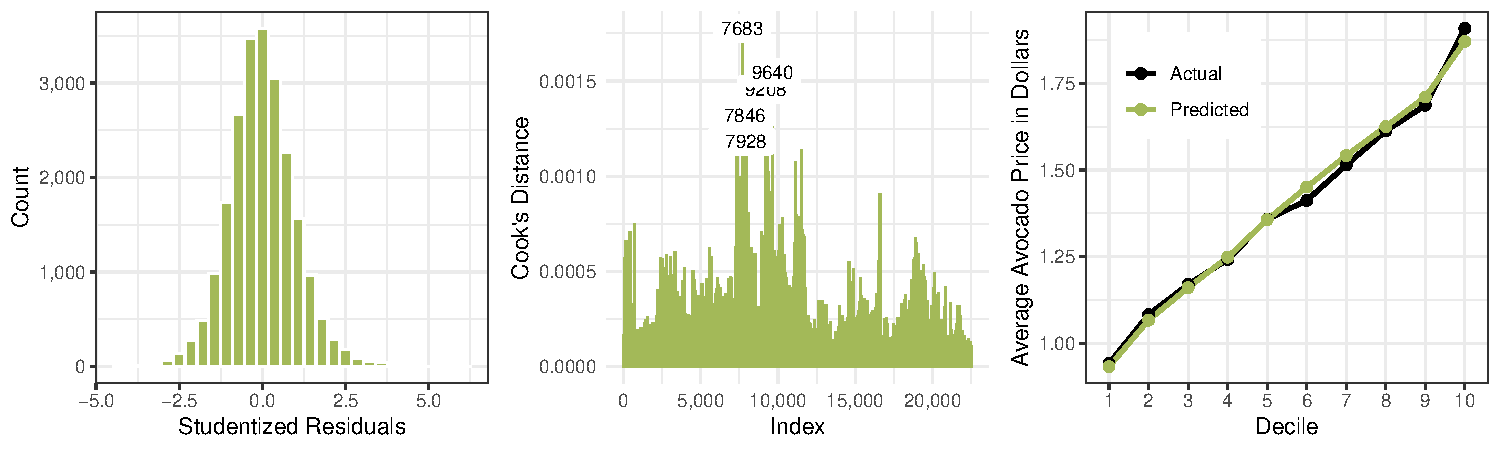
\includegraphics[width=\maxwidth]{figure/unnamed-chunk-4-1} 

\caption{}
\label{diag1}
\end{center} 
\end{figure}

\noindent Cook's distance is also one of the most important criteria to check the influential points wih respect to the predictors. If Cook's distance for an observation is relative high, this observation could be an influential point. Figure~\ref{diag1}.2 depicts a Cook's distance plot for each observation point in the training data. All points are mostly smaller than 0.0005. However, there are five extremely high Cook's distance that needed attention include 7928, 7846, 7683, 9208, and 9640. These values are influential points that originated from independent variables. As seen in Table~A\ref{outliers_table}, total number of avocados sold should be higher in the first half of the year. However, none of the observations were decided to remove from the data since there are no sufficient reasons to remove them. Last but not least, the VIF scores was generated to check if there is any multicolineary issue presented in the model. However, there are no signal saying that there would be multicolinarity issues in the model. Table~A\ref{vif_table} shows all VIF values are below 2 which indicate there are no multicolinearity issues. 

\noindent A .25 proportion of data was hold out to use as a test set to validate the model. After genearting prediction, an MSE score was computed to be approximately 0. This indicates the model is predicting really well with an overall mean square error of nearly 0. To further prove this point, a lift chart was constructed. The predicted average avocado price was sorted from smallest to higher then divided into 10 equal deciles. The actual and predicted average price was computed by decile to compare. Figure~\ref{diag1}.3 shows a lift chart of empirical and indicated values of average avocado price. In this plot, the two lines are very closed to each other consistent with the model is robust. Therefore, this model can be use to predict the price of avocados.   
\hfill \break


\noindent Now that we have built the model and checked the quality of the model, an interpretation of the model will be present in this section. All values mentioned in this section are from Table~\ref{final_fit}. The final model is consisted of four variables including total number of avocado sold, month of observation, avocado type, and geographical group. This model has an adjusted R-squared of 0.57 indicating that 57\% of the data in the target variable can be explained by four predictors. Total volume has a negative relationship with total average price, according to the model. On average, if total number of avocado sold increases by one percent, the average price will decreases by \$0.0003. Moreover, the month of observation also have signficant impact on the price of avocado. As mentioned before, avocados would be cheaper during avocado seasons. Different months of the year would generate a different revenue for avocados. For example, February would have lower avocado price than January by 0.037 times, while March has higher avocado price than January by 0.031 times. The values for the rest of the months can be retrieved at Table~\ref{final_fit}. Moving on to the next variable avocado type. How the avocados grow have greately impacted the price of the avocados. An organic avocado would increase the avocado price by 0.367 times compared to conventional avocado. This makes sense because the money goes with the quality. Last but not least, the region of where the avocados were sold are also a significant factor in the model. Regions and cities for each geographical group can be found in Table~A\ref{region}. In general, if an avocado is sold from region 2, the price of avocado inreases by 0.160 times compared to region 1. In addition, the price would increase by 0.309 and 0.0563 times if an avocado is sold from region 3 and 4, respectively, compared to region 1.
\hfill \break


\noindent\textbf{\underline{Conclusion}}: 
\hfill \break


\clearpage
\noindent\textbf{\underline{Bibliography}}:
\hfill \break


\clearpage
\newpage
\noindent \Large{{\bf Appendix A: Supplemental Tables}}

\begin{center}

% Table created by stargazer v.5.2.2 by Marek Hlavac, Harvard University. E-mail: hlavac at fas.harvard.edu
% Date and time: Sun, Dec 13, 2020 - 8:54:08 PM
\begin{table}[H] \centering 
  \caption{Summary Statistics for all numerical independent features} 
  \label{desc_stat_ind} 
\begin{tabular}{@{\extracolsep{5pt}}lccccccc} 
\\[-1.8ex]\hline 
\hline \\[-1.8ex] 
Statistic & \multicolumn{1}{c}{N} & \multicolumn{1}{c}{Mean} & \multicolumn{1}{c}{St. Dev.} & \multicolumn{1}{c}{Min} & \multicolumn{1}{c}{Pctl(25)} & \multicolumn{1}{c}{Pctl(75)} & \multicolumn{1}{c}{Max} \\ 
\hline \\[-1.8ex] 
total\_volume & 30,021 & 939,255 & 3,813,519 & 85 & 14,299 & 489,803 & 63,716,144 \\ 
4046 & 30,021 & 299,107 & 1,289,108 & 0 & 783 & 115,156 & 22,743,616 \\ 
4225 & 30,021 & 284,901 & 1,169,078 & 0 & 2,814 & 140,947 & 20,470,573 \\ 
4770 & 30,021 & 21,629 & 100,919 & 0 & 0 & 5,424 & 2,546,439 \\ 
total\_bags & 30,021 & 333,534 & 1,415,618 & 0 & 8,374 & 159,174 & 31,689,189 \\ 
small\_bags & 30,021 & 232,126 & 950,503 & 0 & 5,956 & 112,938 & 20,550,407 \\ 
large\_bags & 30,021 & 95,185 & 467,210 & 0 & 352 & 36,068 & 13,327,601 \\ 
xlarge\_bags & 30,021 & 6,223 & 38,137 & 0 & 0 & 560 & 1,022,564 \\ 
\hline \\[-1.8ex] 
\end{tabular} 
\end{table} 

\end{center}

\begin{center}
% latex table generated in R 3.6.2 by xtable 1.8-4 package
% Sun Dec 13 20:54:09 2020
\begin{table}[ht]
\centering
\begin{tabular}{rp{1.5in}p{.8in}llll}
  \hline
 & Model & Number of Features & MSE & Adj.R.squared & F.statistics & AIC \\ 
  \hline
1 & Initial Model & 16.000 & 0.062 & 0.572 & 1879.873 & 1421.841 \\ 
  2 & Stepwise Model & 16.000 & 0.062 & 0.572 & 1879.873 & 1421.841 \\ 
  3 & Model with Interaction Terms & 78.000 & 0.060 & 0.588 & 413.437 & 598.507 \\ 
  4 & Stepwise Model with Interaction Terms & 77.000 & 0.060 & 0.588 & 418.808 & 597.053 \\ 
   \hline
\end{tabular}
\caption{Regression validation metrics including MSE, R-squared adjusted, and AIC} 
\label{reg_vali_metric}
\end{table}

\end{center} 


\begin{center}
% latex table generated in R 3.6.2 by xtable 1.8-4 package
% Sun Dec 13 20:54:09 2020
\begin{table}[ht]
\centering
\begin{tabular}{rrrrlll}
  \hline
 & Index & average\_price & log\_total\_volume & month & type & geography\_bins \\ 
  \hline
1 & 7339 & 3.030 & 8.220 & 10 & organic & 2 \\ 
  2 & 7683 & 3.250 & 9.723 & 10 & organic & 4 \\ 
  3 & 7846 & 2.990 & 9.849 & 11 & organic & 4 \\ 
  4 & 7928 & 2.940 & 9.766 & 11 & organic & 4 \\ 
  5 & 9208 & 3.050 & 7.634 & 3 & organic & 2 \\ 
  6 & 9640 & 3.170 & 8.013 & 4 & organic & 2 \\ 
  7 & 11523 & 2.990 & 7.944 & 10 & organic & 2 \\ 
   \hline
\end{tabular}
\caption{} 
\label{outliers_table}
\end{table}

\end{center} 



\begin{center}
% latex table generated in R 3.6.2 by xtable 1.8-4 package
% Sun Dec 13 20:54:09 2020
\begin{table}[ht]
\centering
\begin{tabular}{rrrr}
  \hline
 & GVIF & Df & GVIF\verb|^|(1/(2*Df)) \\ 
  \hline
log\_total\_volume & 2.713 & 1.000 & 1.647 \\ 
  month & 1.007 & 11.000 & 1.000 \\ 
  type & 2.673 & 1.000 & 1.635 \\ 
  geography\_bins & 1.031 & 3.000 & 1.005 \\ 
   \hline
\end{tabular}
\caption{} 
\label{vif_table}
\end{table}

\end{center} 


\begin{center}
% latex table generated in R 3.6.2 by xtable 1.8-4 package
% Sun Dec 13 20:54:09 2020
\begin{table}[ht]
\centering
\begin{tabular}{rll}
  \hline
 & geography & geography\_bins \\ 
  \hline
1 & Cincinnati/Dayton & 1 \\ 
  2 & Columbus & 1 \\ 
  3 & Dallas/Ft. Worth & 1 \\ 
  4 & Houston & 1 \\ 
  5 & Nashville & 1 \\ 
  6 & New Orleans/Mobile & 1 \\ 
  7 & Phoenix/Tucson & 1 \\ 
  8 & Roanoke & 1 \\ 
  9 & South Central & 1 \\ 
  10 & Atlanta & 2 \\ 
  11 & Buffalo/Rochester & 2 \\ 
  12 & Denver & 2 \\ 
  13 & Detroit & 2 \\ 
  14 & Great Lakes & 2 \\ 
  15 & Harrisburg/Scranton & 2 \\ 
  16 & Indianapolis & 2 \\ 
  17 & Jacksonville & 2 \\ 
  18 & Las Vegas & 2 \\ 
  19 & Los Angeles & 2 \\ 
  20 & Louisville & 2 \\ 
  21 & Miami/Ft. Lauderdale & 2 \\ 
  22 & Midsouth & 2 \\ 
  23 & Orlando & 2 \\ 
  24 & Pittsburgh & 2 \\ 
  25 & Plains & 2 \\ 
  26 & Portland & 2 \\ 
  27 & Richmond/Norfolk & 2 \\ 
  28 & South Carolina & 2 \\ 
  29 & Southeast & 2 \\ 
  30 & Tampa & 2 \\ 
  31 & Total U.S. & 2 \\ 
  32 & West & 2 \\ 
  33 & West Tex/New Mexico & 2 \\ 
  34 & Albany & 3 \\ 
  35 & Baltimore/Washington & 3 \\ 
  36 & Boise & 3 \\ 
  37 & Boston & 3 \\ 
  38 & California & 3 \\ 
  39 & Charlotte & 3 \\ 
  40 & Chicago & 3 \\ 
  41 & Grand Rapids & 3 \\ 
  42 & Northeast & 3 \\ 
  43 & Northern New England & 3 \\ 
  44 & Philadelphia & 3 \\ 
  45 & Raleigh/Greensboro & 3 \\ 
  46 & Sacramento & 3 \\ 
  47 & San Diego & 3 \\ 
  48 & Seattle & 3 \\ 
  49 & Spokane & 3 \\ 
  50 & St. Louis & 3 \\ 
  51 & Syracuse & 3 \\ 
  52 & Hartford/Springfield & 4 \\ 
  53 & New York & 4 \\ 
  54 & San Francisco & 4 \\ 
   \hline
\end{tabular}
\caption{} 
\label{region}
\end{table}
% latex table generated in R 3.6.2 by xtable 1.8-4 package
% Sun Dec 13 20:54:09 2020
\begin{table}[ht]
\centering
\begin{tabular}{rrrr}
  \hline
 & GVIF & Df & GVIF\verb|^|(1/(2*Df)) \\ 
  \hline
log\_total\_volume & 2.713 & 1.000 & 1.647 \\ 
  month & 1.007 & 11.000 & 1.000 \\ 
  type & 2.673 & 1.000 & 1.635 \\ 
  geography\_bins & 1.031 & 3.000 & 1.005 \\ 
   \hline
\end{tabular}
\caption{} 
\label{vif_table}
\end{table}

\end{center} 


\clearpage
\newpage
\noindent \Large{{\bf Appendix B: Supplemental Figures}}

\begin{figure}[h!] 
\begin{center}

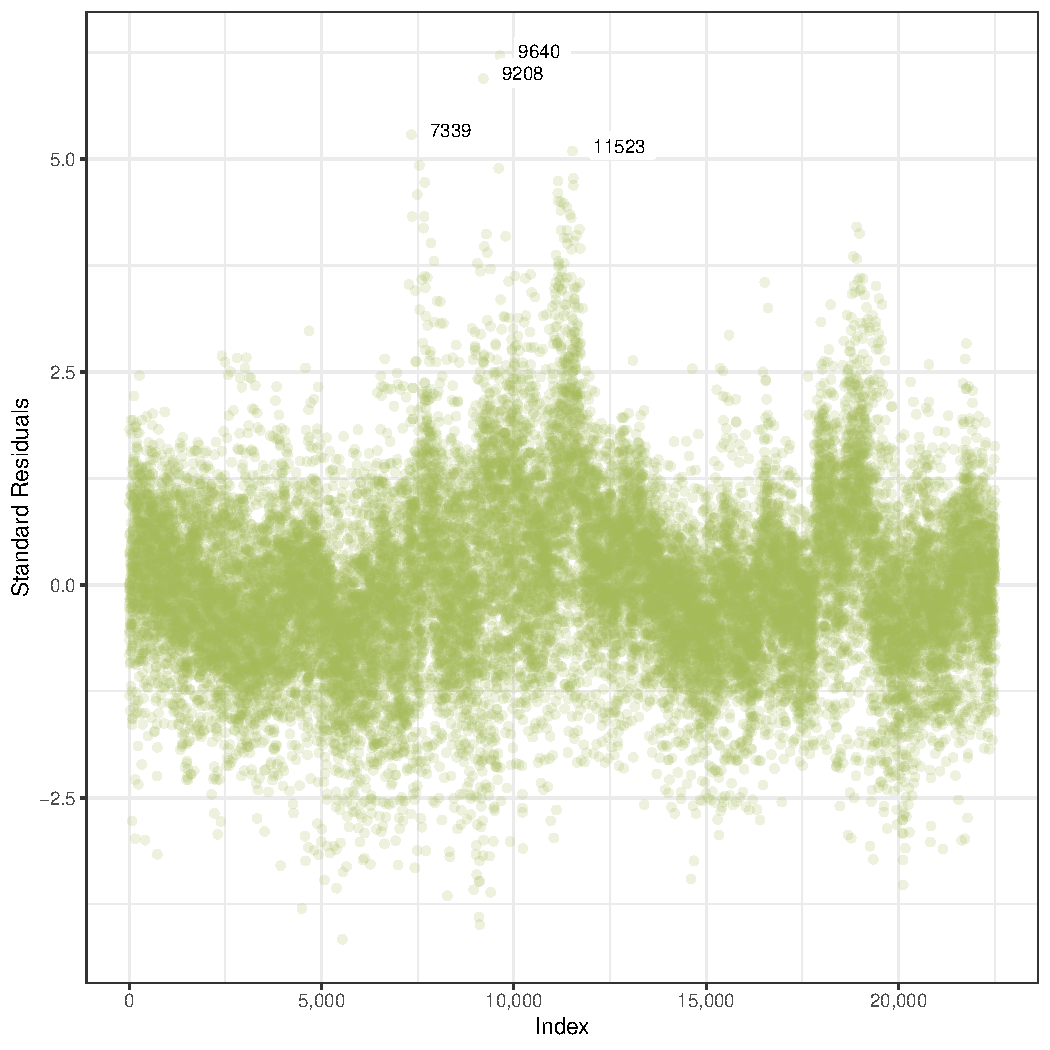
\includegraphics[width=\maxwidth]{figure/unnamed-chunk-10-1} 

\caption{}
\label{diag3}
\end{center} 
\end{figure}


\clearpage
\newpage
\noindent \Large{{\bf Appendix C: R Code}}
\lstinputlisting[language=R, caption = Appendix of Code]{R/dar3-codes.R}


\end{document}






